\documentclass{article}
\usepackage{preamble}
%\usepackage{subfig}
\newcommand{\dblspace}{\setlength{\baselineskip}{0.8cm}}
\renewcommand{\pskinny}[2]{p\big(#1|#2\big)}
\usepackage{graphicx} % For figures
\usepackage{subfigure} 
\usepackage{natbib}   % For citations
\usepackage{algorithm}
\usepackage{algorithmic}
\usepackage{hyperref}
\newcommand{\theHalgorithm}{\arabic{algorithm}}
\usepackage[normalem]{ulem}  % for strikethrough
\usepackage{color} % for comments to each other
\usepackage{comment}
\usepackage{pgfplots}
\usepackage{icml2012}

% The width of one column in cm: \printinunitsof{cm}\prntlen{\columnwidth} = 8.25381

% \usepackage[accepted]{icml2012}¡

% The \icmltitle you define below is probably too long as a header.
% Therefore, a short form for the running title is supplied here:
\icmltitlerunning{Sampling for Bayesian Quadrature}

\begin{document} 
\twocolumn[
\icmltitle{
Bayesian Quadrature for Active Learning of Model Evidence}
%Sampling for Bayesian Quadrature\\or\\Actively Learning Normalization Constants\\or\\Doubly Bayesian Quadrature: The \acro{bbq} Algorithm\\or\\

% It is OKAY to include author information, even for blind
% submissions: the style file will automatically remove it for you
% unless you've provided the [accepted] option to the icml2012
% package.
\icmlauthor{Your Name}{email@yourdomain.edu}
\icmladdress{Your Fantastic Institute,
            314159 Pi St., Palo Alto, CA 94306 USA}
\icmlauthor{Your CoAuthor's Name}{email@coauthordomain.edu}
\icmladdress{Their Fantastic Institute,
            27182 Exp St., Toronto, ON M6H 2T1 CANADA}

% You may provide any keywords that you 
% find helpful for describing your paper; these are used to populate 
% the "keywords" metadata in the PDF but will not be shown in the document
\icmlkeywords{Bayesian Quadrature, Monte Carlo, Gaussian Processes, Numerical Integration, Model Evidence, Likelihood ratios}

\vskip 0.3in
]

\begin{abstract} 
%We describe a novel approach to quadrature for probabilistic integrals, offering a competitor to traditional Monte Carlo methods. We use a Bayesian quadrature framework \citep{BZHermiteQuadrature,BZMonteCarlo}.
We introduce several innovations making Bayesian Quadrature methods suitable for computing model evidences, or normalization constants.  We demonstrate several advantages of model-based integration over standard Monte Carlo approaches.  These include sample efficiency, and an estimate of the uncertainty in our integral. We extend existing Gaussian process models by modeling the non-negativity of our integrand, and by approximately marginalising over hyperparameters in closed form.  We use active learning to select our function samples, as opposed to running a Markov chain.
\end{abstract} 

\section{Introduction}

The quadrature problem 
\begin{equation}\label{eq:Y}
Y = \int f(\vlfv) p(\vlfv) d\vlfv
\end{equation}
is both common and important.  In machine learning applications, the quadrature problem often appears when evaluating integrals over probabilities
\begin{equation}\label{eq:ev}
Z = \int \ell(\vlfv) p(\vlfv) d\vlfv
\end{equation}
where $\ell(\vlfv)$ is non-negative.  Examples of this problem appear when computing marginal likelihoods, partition functions, predictive distributions at test points, or when marginalizing over variables in a model.  In this paper, we focus on computing model evidences, where $\ell(\vlfv)$ is the unnormalized likelihood of some parameters $x_1 \dots x_D$.

%Training or evaluating any probabilistic model typically requires an integration over model parameters, weighted by their likelihoods.  This common problem has many names:  computing the model evidence, calculating the marginal likelihood, estimating the partition function or normalizing a distribution.  Typically, this task is performed using Markov-Chain Monte Carlo (\acro{mcmc}) methods.  These methods have many well-known problems, such as requiring extensive tuning, becoming stuck in local modes, and falsely appearing to converge \citep{NealMC}.  However, almost all standard approaches fall into the wide family of \acro{mcmc} methods.

There exist several standard randomized methods for computing model evidence, such as annealed importance sampling (\acro{ais}) \citep{neal2001annealed}, nested sampling \citep{skilling2004nested} and bridge sampling.  For a review, see \citet{chen2000monte}.   These methods estimate $Z$ given the value of the integrand on a set of sample points, whose size is limited by the expense of evaluating $\ell(\vlfv)$.  It is well-known that convergence diagnostics for Monte Carlo estimates of partition functions are often unreliable \citep{NealMC, brooks1998convergence, cowles1999possible}.  As well, most sophisticated randomized algorithms have parameters which must be set by hand, such as proposal distributions or temperature schedules.

%\section{Model-Based Integration}

An alternative, model-based approach, Bayesian Quadrature \citep{BZHermiteQuadrature}, specifies a distribution over likelihood functions, using observations of the likelihood to infer a distribution for $Z$ (see Figure \ref{fig:model_based}). Bayesian Quadrature has previously been used to infer model evidence, \citep{BZMonteCarlo}.  We improve upon this work in three ways:

\begin{figure}
\centering
\psfragfig[width=\columnwidth]{figures/bmc_intro}
\caption{An illustration of model-based integration.  We compute the expected area underneath a distribution over functions, conditioned on sampled values of the true function.  Samples added at new locations will reduce our uncertainty about the area under the function.}
\label{fig:model_based}
\end{figure}

%As discussed in \citep{MCUnsound}, traditional Monte Carlo integration techniques do not make the best possible use of this valuable information. An alternative is found in Bayesian quadrature (\acro{bq}) \citep{BZHermiteQuadrature}, a method which uses function samples within a Gaussian process model to compute a closed-formed posterior over the value of the integral.



\paragraph*{Log-prior:} Previous work used a \gpb prior on the likelihood function, which is a poor model since it cannot express the non-negativity and high dynamic range of most likelihood function.  We introduce tractable approximate inference under a log-\gp, which properly captures these properties of likelihood functions.

%Our problem is to estimate the evidence of some model $M$. This is computed as 
%\begin{equation}\label{eq:ev}
% Z = p(M) = \int l(x) p(x) dx\,,
%\end{equation}
%for the likelihood $l(x) = \p{M}{x}$. The arguments $x$ represent the appropriate parameters of the model, which must be marginalised. 
%Unfortunately, the integral is typically non-analytic for interesting likelihood functions. 

\paragraph*{Active Sampling:} In \citep{BZMonteCarlo}, sample points were chosen in a randomized manner.  We demonstrate how to actively choose sample points in order to minimize the uncertainty in our integral.

\paragraph*{Hyperparameter Marginalisation:} Uncertainty in the quadrature hyperparameters has previously been ignored, leading to overconfidence in the estimate of $Z$.  We introduce a tractable approximate marginalization of lengthscale hyperparameters.


%\paragraph*{Convergence:} Here the issue of convergence is solved naturally: our posterior variance over $Z$ indicates the uncertainty remaining in the quantity we care about. 

We compare our \acro{bq} approach to standard Monte Carlo techniques on both simulated and real scientific problems, where we demonstrate one of the key advantages of \acro{bq}: a closed-form expression for the posterior uncertainty over $Z$ provides a natural convergence diagnostic.

%\section{Estimating Model Evidence}\label{sec:ev}

%Here, we give a brief overview of the standard methods used for computing normalization constants.  For the remainder of the paper, we will assume that we are able to draw samples from 

%Our problem is to estimate the evidence of some model $M$. This is computed as $$Z = p(M) = \int l(x) p(x) dx\,,$$ for the likelihood $l(x) = \p{M}{x}$. The arguments $x$ represent the appropriate parameters of the model, which must be marginalised. 
%Unfortunately, the integral is typically non-analytic for interesting likelihood functions. 

%\paragraph*{Annealed Importance Sampling} \citep{neal2001annealed} is a popular thermodynamic integration method which 
%These typically involve the construction of a markov chain for generating samples, leading to them being termed \emph{Markov chain Monte Carlo} (\acro{mcmc}) methods. 

%One of the main difficulties with using \acro{mcmc} methods in practice is that most methods have at least a handful of parameters which are typically set by hand. These often include a `burn-in' parameter, specifying a certain quantity of data to exclude when constructing the final estimate. The selection of this parameter can be problematic \citep{cowles1999possible}. 

%Convergence diagnostics exist to indicate if a Markov chain is failing to `mix', or explore the entire integrand.  However, these methods are known to have failure modes in which diagnostics do not identify a lack of mixing \citep{NealMC, brooks1998convergence, cowles1999possible}. One solution to this problem is found by `exact' or `perfect' sampling via coupling from the past \citep{green1999exact}, but is impractical for realistic problems. 

%While standard errors are possible for \acro{mcmc}, typically they rely on the sampler mixing well \citep{flegal2008markov}. As such, these errors can not identify exactly the failure to mix that is of most concern. The distribution of most use for our inference is a Gaussian process, which we now briefly introduce. 

\section{Gaussian Processes}
Gaussian processes (\gp s) offer a powerful method to perform Bayesian inference about functions \citep{GPsBook}. A \gpb is defined as a distribution over the functions $f: \mathcal{X} \rightarrow \mathbb{R}$ such that the distribution over the possible function values on any finite subset of $\mathcal{X}$ is multivariate Gaussian. For clarity, we'll henceforth assume $\mathcal{X} = \mathbb{R}$, although all results generalise readily to $\mathbb{R}^n$. For a function $f(\lfv)$, the prior distribution over its values $\vf$ on $\vlfv \subset \mathcal{X}$ is
\begin{align}%\label{eq:\gpbDefn}
\textstyle
 &\po{\vf}\deq \N{\vf}{\vmu}{K}\\
 &\deq\frac{1}{\sqrt{\det{2\pi K}}}\,\exp \big(-\frac{1}{2}\,(\vf-\vmu)\tra\,K\inv\,(\vf-\vmu)\big),
\end{align}
This distribution is specified by mean and covariance functions, which generate mean vector $\vmu_{f}$ and covariance matrix $K_{f}$ respectively. 
In this paper, we'll use Gaussian (squared exponential) covariance functions,
\begin{align} \label{eq:Gaussian_cov_fn}
% K(\vlfv,\vlfv') & \deq \prod_{e=1}^{E} K_e\big(\phi\pha_e,\phi_e'\big)\\
\textstyle
K_{f}(\lfv_1,\lfv_2)& \deq h_f^2\,\N{\lfv_1}{\lfv_2}{w_{f}}.
\end{align} 
Here $h_f$ specifies the output scale (`height') over $f$, while $w_f$ defines a (squared) input scale (`width') over $\lfv$. Note that if $x$ has dimension greater than one, $w_f$ is a covariance matrix; we'll assume $w_f$ is diagonal. 

Given observations $(\vlfv_s,\vf_s)$, we are interested in making predictions about  $f_\star$ at input $\lfv_\star$. We will assume that function inputs such as $\vlfv_s$ and $\lfv_\star$ are always known; they will not be explicitly represented. With this information, we have the predictive equations
\begin{equation}
 \pskinny{f\st}{\vf_s} = 
\bN{f\st}
{\meancond{f}{\vlfv_\star}{s}}
{\covcond{f}{\vlfv_\star}{s}}\,,
\end{equation}
where the mean $m$, covariance $C$, and variance $V$ are
\begin{align} 
\textstyle
&\meancond{f}{\lfv_\star}{s}
\deq \mean{f_\star}{\vf_s}
\nonumber\\
&= \mu_{f}(\lfv_\star)\!+\!
K_{f}(\lfv_\star,\vlfv_s)
K_{f}(\vlfv_s,\vlfv_s)\inv\!
\bigl(\vf_s\!-\!{\mu}_{f}(\vlfv_s)\bigr)\label{eq:GPMean}
\end{align} 
\begin{align}
&C_{f|s}(\lfv_\star, \lfv'_\star)
\deq C(f_\star,f'_\star|\vf_s) 
\nonumber\\
&=\!K_{f}(\lfv_\star,\lfv'_\star)\! - \!
K_{f}(\lfv_\star,\!\vlfv_s)
K_{f}(\vlfv_s,\!\vlfv_s)\inv\!
K_{f}(\vlfv_s,\!\lfv'_\star)%\label{eq:\gpbCov}
\\[0.2cm]
&\covcond{f}{\lfv_\star}{s}
\deq {\cov{f_\star}{\vf_s}} 
\deq C_{f|s}(\lfv_\star, \lfv_\star).
\end{align} 
Note that the above assumes implicit conditioning on hyperparameter. Where required for disambiguation, we'll make this explicit, as per $m_{f|s,w_f}(x\st) \deq \mean{f\st}{\vf_s, w_f}$ and so forth.

\section{Bayesian Quadrature} \label{sec:bq}

% Note that maximum likelihood is also subject to issues. $\p{D}{\lfv,I}$, how come (known) $I$ is on the right and (known) $D$ is on the left? 

\emph{Bayesian quadrature} \citep{BZHermiteQuadrature,BZMonteCarlo} is a means of performing Bayesian inference about the value of a potentially nonanalytic integral \eqref{eq:Y}.
%Note that we use a condensed notation; this and all integrals to follow are definite integrals over the entire domain of interest.
We'll assume we are integrating with respect to a Gaussian prior
$\po{\lfv} \deq \N{\lfv}{\nu_{\lfv}}{\lambda_{\lfv}}$,
although other convenient forms, or, if necessary, the use of an importance re-weighting trick, allow any other integral to be approximated. If $\lfv$ is a vector, $\nu_{\lfv}$ is a  vector of identical size, and $\lambda_{\lfv}$ an appropriate covariance matrix.

%\textcolor{red}{[I'm hoping to re-write the next two paragraphs; it's way too indirect, and I think the philosophical foundations of \acro{mcmc} are a poor avenue of attack]}
Quadrature involves evaluating $f(\lfv)$ at a vector of sample points $\vlfv_s$, giving $\vf\pha_s\deq f(\vlfv_s)$. Often this evaluation is computationally expensive; the consequent sparsity of samples introduces uncertainty about the function $f$ between them, and hence uncertainty about the integral $Y$.

%As ever in the face of uncertainty, we address the estimation of the value of our integral as a problem of Bayesian inference \citep{BZNumericalAnalysis}. 

%In considering any problem of inference, we need to be clear about both what information we have and which uncertain variables we are interested in. In our case, both the values $f(\vlfv_s)$ and their locations $\vlfv_s$ represent valuable pieces of knowledge. As discussed by \citet{MCUnsound}, traditional Monte Carlo, which approximates as
%\begin{equation} \label{eq:MC_integral_estimate}
%\inty{f} \simeq \frac{1}{\card{s}} \sum_{i=1}^{\card{s}} f(\lfv_i)\,,
%\end{equation}
%effectively ignores the information content of $\vlfv_s$, leading to unsatisfactory behaviour.
%\footnote{  For example, imagine that we had $\card{s}=3$, and $\lfv_1 = \lfv_2$. In this case, the identical value $q(\lfv_1)= q(\lfv_2)$ will receive $\nicefrac{2}{3}$ of the weight, whereas the equally useful $q(\lfv_3)$ will receive only $\nicefrac{1}{3}$. \textcolor{red}{I'm not crazy about this argument, since the weightings are also incorporating information about the prior...} }

Traditional Bayesian quadrature chooses a \gpb prior for $f$, with mean $\mu_f$ and the Gaussian covariance \eqref{eq:Gaussian_cov_fn}. Here the scales $h_f$ and $w_f$ are \emph{quadrature hyperparameters}, hyperparameters that specify the  \gpb used for Bayesian quadrature. These scales are typically fitted using maximum likelihood; we will later introduce an approximate means of marginalising them in Section \ref{sec:marginalizing}.

% Many more of these will be implicitly introduced in the coming sections; we'll take this as given and incorporate them into the (hidden) context $I$. 
% Note that it will later become apparent that our inference for $\inty{f}$ is independent of the $h_f$ quadrature hyperparameter.

Note that variables possessing a multivariate Gaussian distribution are jointly Gaussian distributed with any affine transformations of those variables. Because integration is affine, we can hence use computed samples $\vf_s$ to perform analytic Gaussian process inference about the value of integrals over $f(\lfv)$, such as $Y$. The mean estimate for $Y$ given $\vf_s$ is
%
\begin{align} \label{eq:mean_inty_f}
\mean{Y}{\vf_s}
& 
=\iint Y\,\p{Y}{f}\p{f}{\vf_s} \ud Y \,\ud f                                                                                                                                                               \nonumber\\
&
 =\iint Y\,\dd{Y}{\int f(\lfv)\,\po{\lfv}\,\ud\lfv}
\nonumber\\
&\hspace{2.5cm}
\N{f}{\meancondfn{f}{s}}{C_{f|s}} \ud Y \,\ud f \nonumber\\
&
 = \int \meancondfn{f}{s}(\lfv)\,\po{\lfv}\,\ud\lfv\nonumber\\
&
 = 
%\N{\inty{f}}
\mu_f + \ntT{s}{f}\, \dtt{s}{f}
%{\varpi_{f}-\ntT{s}{f} K_{f}(\vlfv_s,\vlfv_s)\inv \nt{s}{f}}
\,,
\end{align}
where for $\lfv_i \in \vlfv_s$,
\begin{align}
\fnt{\lfv_i}{f} & \deq \!\int K_f(\lfv_i,\lfv)\po{\lfv}\ud\lfv
 = h_f^2\,\N{\lfv_i}{\nu_{\lfv}}{\lambda_{\lfv}+w_{f}}\nonumber\\
%\intertext{and}
\dtt{s}{f} & \deq K_{f}\bigl(\vlfv_s,\vlfv_s\bigr)\inv (\vf_s-{\mu}_{f})\,.
\end{align}
%
%Note that the form of our `best estimate' for $\inty{f}$, \eqref{eq:mean_inty_f}, is an affine combination of the samples $\vf_s$, just as for traditional quadrature or Monte Carlo techniques. 
% Indeed, if $\mu_f$ is taken as the mean of $\vf_s$ (as is usual for \gpb inference), the second term in \eqref{eq:mean_inty_f} can be viewed as a correction factor to the Monte Carlo estimate \eqref{eq:MC_integral_estimate}. \textcolor{red}{[Since we're using a different sampling strategy than \acro{mcmc} in this paper, I think the preceeding statement is kind of misleading / confusing...]}
% \sout{Note also that $h_f$ represents a simple multiplicative factor to both $\ntT{s}{f}$ and $K_{f}\bigl(\vlfv_s,\vlfv_s\bigr)$, and as such cancels out of \eqref{eq:mean_inty_f}.} 
%
Its variance is also readily computed. Similarly, we can compute the posteriors for integrals over the product of multiple, independent functions. For example, we can calculate the posterior mean 
$\mean{\inty{f g}}{\vf_s, \vect{g}_s}$ for an integral $\int f(x) g(x) \ud x$. 
 In the following three sections, we will expand upon the improvements this paper introduces in the use of Bayesian Quadrature for computing model evidences.

\section{Modeling Likelihood Functions}\label{sec:model_lik}

We wish to evaluate the evidence \eqref{eq:ev}, an integral over non-negative likelihoods, $\lfn(\lfv)$.
%
 \begin{figure}
 \centering
 \psfragfig[width=\columnwidth]{figures/log_transform}
 \caption{The lengthscale of a \gpb fitted to the log-likelihood function will typically be much longer than that of a \gpb fit to the likelihood function.  A \gpb with a long lengthscale will generalize better to distant parts of the function, and will have a posterior more concentrated around the true evidence. }
 \label{fig:log_is_better}
 \end{figure}
%
\begin{figure}
\centering
\psfragfig{figures/delta}
\caption{An illustration of our method of finding the integral under the exp of a Gaussian process.}
\label{fig:delta}
\end{figure}
%
Assigning a standard \gpb prior to $\lfn(\lfv)$ would ignore prior information about the range and non-negativity of $\lfn(\lfv)$, leading to pathologies such as potentially negative evidences (as observed in \citet{BZMonteCarlo}).  A much better prior would be a \gpb prior on $\log\bigl(\lfn(x)\bigr)$ (see Figure \ref{fig:log_is_better}). However, the integral under the exp of a \gpb is intractable,
% 
\begin{multline}\label{eq:minty_l}
\mean{\If}{\vr_s}
% & 
% =\iint \inty{l}\,\p{\inty{l}}{l}\p{l}{\vl_s} \ud \inty{l} \,\ud l                                                                                                                                                               \nonumber\\
% &
 =\int \Bigl( \int \exp\bigl(\tr(\lfv)\bigr)\po{\lfv}\,\ud\lfv\Bigr)\\
\N{\tr}{\meancondfn{\tr}{s}}{C_{\tr|s}} \ud \tr\,.
\end{multline}
%
Here the exponential ruins the linearity that yielded the analyticity in Section \ref{sec:bq}. To combat this, we adopt the approximate inference method of \citep{BQR} to tractably integrate under a log-\gpb prior.\footnote{In practice, we use the transform 
$\log\left(\lfn(\lfv) + 1\right)$, allowing us to assume the transformed quantity has zero mean. For the sake of simplicity, we omit this detail in the following derivations.} That is, we perform inference for $Z$ directly as a functional of $\tr$;
%
\begin{align}
 Z[\tr] & = \int \exp \bigl( \tr(\lfv)\bigr) p(\lfv) \ud \lfv\\
  						    %& = \int \lfn(\lfv) p(\lfv) \ud \lfv\\
\pderiv{}{\tr(\lfv)}Z[\tr] & = \exp \bigl( \tr(\lfv)\bigr) p(\lfv) % = \lfn(\lfv) p(\lfv)
\,.
\end{align}
%
We now make a \emph{linearisation} approximation\footnote{Note that this linearisation is equivalent to taking another \gpb for $Z$. with the affine covariance
\begin{equation}
 K_Z(\tr,\tr')
% \deq 
%  K_Z\bigl((\tvq\pha_c,\tvr\pha_c),(\tvq'_c,\tvr'_c)\bigr)
\deq
\int\tr(\lfv) \tr'(\lfv) \ud \lfv
+ \omega^2\,.
\end{equation}
} 
for $Z$, assuming $Z$ to be affine in $\tr$. 
Note that \eqref{eq:minty_l} consists of the product of $Z[\tr]$ and a \gpb for $\tr$; the latter, due to the light tails of the Gaussian, effectively permits only a small range of $\tr$ functions. Over this narrow region, it is reasonable to assume that $Z[\tr]$ does not vary too dramatically, and can be approximated as linear. If we perform the linearisation of $Z[\tr]$ around a point defined by $\tr_0$, we can define terms required for linearisation
$Z_0 \deq Z[\tr_0]$ and $\pderiv{Z_0}{\tr(\lfv)} \deq \pderiv{Z}{\tr(\lfv)}[\tr_0]$.  Linearisation then gives us
\begin{equation}\label{eq:linearisation}
\novmean{Z[\tr]}{Z_0,\pderiv{Z_0}{\tr(\lfv)}, \tr} 
= Z_0+\varepsilon[\tr],
\end{equation}
where
\begin{equation} \label{eq:correction}
\varepsilon[\tr] \deq \int \pderiv{Z_0}{\tr(\lfv)}\bigl(\tr(\lfv)-\tr_0(\lfv)\bigr)\ud\lfv\,.
\end{equation}
As with any linearisation approximation, \eqref{eq:linearisation} gives the value at the selected point $\tr_0$, plus a correction factor $\varepsilon$ modeling the influence of the first derivatives.

We choose $\tr_0$ so as to resolve the non-analytic integrals required:  $\tr_0 \deq \log (m_{\lfn|s})$. This involves the introduction of a separate \gpb model over $\lfn$, the non-log space.  Then $m_{\lfn|s}$ is the \gpb conditional mean (as per \eqref{eq:GPMean}) for $\lfn$ given observations $\lfn(\vlfv_s)$. For this \gpb (over the non-log space), we take zero prior means and Gaussian
covariances of the form \eqref{eq:Gaussian_cov_fn}. 
% Our linearisation corresponds to giving our \gpb over $Z$ observations
% at $\tr_0= \log (m_{r|s})$ of both the functional itself,
We now have
\begin{align}
Z_0 & = Z[\tr_0]
= 
{\mean{\If}{\vr_s}}
\intertext{(which is of the form \eqref{eq:mean_inty_f}) along with the functional derivative}
\hspace{-0.2cm}\pderiv{Z_0}{\tr(\lfv)} & = \pderiv{Z}{\tr(\lfv)}[\tr_0]
 = \mean{\lfn(\lfv)}{\vr_s}\,\po{\lfv}.
\end{align}
Note that $Z_0$ and its functional derivatives are analytic due to our choice of $\tr_0$. 

For brevity, we assume that if we condition on $Z_0$, we will also implicitly condition on its functional derivative. This allows us to write the mean for  $Z$
%
\begin{align}
& \mean{\If}{Z_0,\tvr_s} \nonumber\\
& \deq \int \mean{Z[\tr]}{Z_0,\tr}
\p{\tr}{\tvr_s}\, \ud \tr 
\nonumber\\
& = \mean{Z[m_{\tr|s}]}{Z_0,m_{\tr|s}} \nonumber\\
& = \mean{\If}{\vr_s} + 
\mean{\varepsilon}{Z_0,\tvr_s}
\label{eq:mean_ev1}
\end{align}
where
\begin{align}\label{eq:mean_corrn}
\mean{\varepsilon}{Z_0,\tvr_s} 
& = \iint \mean{\lfn(\lfv)}{\vr_s}\,
\Delta(\lfv)\,\po{\lfv}\ud\lfv\,.
\end{align}
Here we have defined the difference between the \gpb mean over the log-transformed likelihood and the transformed \gpb mean over the original likelihood (illustrated in Figure \ref{fig:delta}) as
\begin{align}
\Delta & \deq m_{\tr |s} - \log(m_{l|s}) = m_{\tr |s}  - \tr_0 \,.
\end{align}
involved in the integral remaining in the correction factor, \eqref{eq:correction}.
We expect $\Delta(\lfv)$ to be everywhere small relative to the magnitude of $\tr(\phi)$ (see Figure \ref{fig:integrate_hypers}). This implies that
 $\tr_0$ is close to the peaks of the Gaussian over $\tr$, rendering our linearisation appropriate. 

Unfortunately, \eqref{eq:mean_corrn} is non-analytic due to the $\tr_0$ term within $\Delta$. As such, we perform another stage of Bayesian quadrature by treating $\Delta$ as an unknown function of $\lfv$. We take Gaussian process priors for $\Delta$, with zero prior mean and Gaussian covariance \eqref{eq:Gaussian_cov_fn}. We must now choose sample points $\vlfv_c$ at which to evaluate the $\Delta$ function. 
Note that we do not need to evaluate $\lfn(\lfv_c)$ in order to compute $\Delta(\lfv_c)$.
% Unfortunately, it is impractical to resolve this decision problem in the same manner as the selection of $\vlfvS$, our ultimate goal (a topic that receives our full attention in Section \ref{sec:S\acro{bq}})).
$\vlfv_c$ should firstly include $\vlfv_s$, where we know that $\Delta$ is equal to zero. Following \citet{BQR}, we select the remainder of $\vlfv_c$  as the  vertices of a Voronoi diagram \citep{okabe1997locational}, where we expect $\delta$ to be extremised. 

Given these samples, we can now marginalise \eqref{eq:mean_ev1} over $\Delta$ to give
\begin{equation} \label{eq:post_mean}
 \hspace{-0.2cm}\mean{\If}{Z_0,\tvr_s,\Delta_c} =
\mean{\If}{\vr_s} + \mean{\inty{\lfn \Delta}}{\vr_s, \Delta_c},
\end{equation}
where the second term, the correction factor, is expected to be small, as $\Delta$ is small. The variance in the evidence is
\begin{align} 
& \cov{\If}{Z_0,\tvr_s,\Delta_c}\nonumber\\ 
& = \secm{\If}{Z_0,\tvr_s} - \mean{\If}{Z_0,\tvr_s,\Delta_c}^2\,,
\end{align}
where the second moment is 
\begin{align}
& \secm{\If}{Z_0,\tvr_s}  \nonumber\\
& \deq \int Z^2 
\delta\bigl(Z - \mean{Z[\tr]}{Z_0}\bigr)
\p{\tr}{\tvr_s}
\ud Z \ud\tr
\nonumber\\
& = \int \mean{Z[\tr]}{Z_0}^2
\N{\tr}{\meancondfn{\tr}{s}}{C_{\tr|s}}
 \ud\tr
\nonumber\\
& = \mean{\inty{\lfn\,C_{\tr|s}\,\lfn}}{\tvr_s}+
\mean{\If}{Z_0,\tvr_s,\Delta_c}^2
\end{align}
and hence 
\begin{align} \label{eq:post_var}
  &\cov{\If}{Z_0,\tvr_s,\Delta_c} = \mean{\inty{\lfn\,C_{\tr|s}\,\lfn}}{\tvr_s} 
\nonumber\\ 
&\deq
 \iint m_{\lfn|s}(\lfv) m_{\lfn|s}(\lfv') C_{\tr|s}(\lfv,\lfv')  p(x) p(x') \ud \lfv \ud\lfv',
\end{align}
which is expressible in closed form, although space precludes us from doing so. This variance can be employed as a convergence diagnostic; it describes our uncertainty in the ultimate quantity of interest.

In summary, we have described a linearisation approach to exploiting a \acro{gp} prior over log-likelihoods to determine the posterior mean \eqref{eq:post_mean} and variance \eqref{eq:post_var} for the evidence. 

\section{Marginalising quadrature hyperparameters}
\label{sec:marginalizing}

We now present a novel means of approximately marginalising the quadrature hyperparameters of the \gpb used to model the log-integrand, $\tr$. In previous approaches to Bayesian Quadrature, quadrature hyperparameters have been fitted using 
 maximum likelihood. However, ignoring the uncertainty in the hyperparameters to which our predictions are sensitive can lead to pathologies. In particular, the reliability of the variance for $Z$ depends crucially upon marginalising over all unknown quantities. 

\begin{figure}
\centering
\psfragfig[width=0.5\textwidth]{figures/int_hypers}
\caption{An illustration of the effect of integrating hyperparameters on the marginal posterior variance.  Regions whose mean varies as the lengthscales changes have an increased marginal posterior variance.}
\label{fig:integrate_hypers}
\end{figure}

The hyperparameters of most interest are the input scales $w$ for the \gpb over the log-likelihood; these hyperparameters can have a powerful influence on the fit to a function. We use maxmimum likelihood to fit all hyperparmeters other than $w$. Unfortunately, the analytic marginalisation of $w$ is ruled out by the complex dependence of our predictions upon these input scales. However, any approximation we make is likely to improve upon the assumption made by maximum likelihood: that the posterior for all hyperparameters is a delta function. We make the following essential assumptions.

 \paragraph*{Flat prior:} We assume that the prior for $w$ is very broad, so that our posterior is a simple scaling of the likelihood. 
\paragraph*{Laplace approximation:} The likelihood of $w$ is taken as Gaussian with mean equal to the maximum likelihood value $\hat{w}$ and with diagonal covariance matrix $C_w$, diagonal elements fitted using the second derivatives of the likelihood.
%the squared input scales $w_s$ of another \gp, fitted to the likelihood $s(w_r)$ of the input scales $w_r$. \textcolor{red}{[Neat idea, but I can think of simple examples where the lengthscale is short but the mass is spread out; it seems to me that it'd be better to first fit a \gpb, then fit a Gaussian to the \gpb posterior.]}
\paragraph*{Affine GP mean:} Given the tightness of the likelihood for $w$, our predictions for $\tr$ are assumed to have a \gpb mean which is affine in $w$ around the maximum likelihood values, and a constant covariance;
\begin{align}
\hspace{-0.2cm} m_{\tr|s,w} & \simeq m_{\tr|s,\hat{w}} 
 + \pderiv{m_{\tr|s,\hat{w}}}{w} (w- \hat{w})\\
 \hspace{-0.2cm} C_{\tr|s, w} & \simeq C_{\tr|s, \hat{w}}.
\end{align}
 
The implication of these assumptions is that the marginal posterior mean over $\tr$ is simply
$
\tilde{m}_{\tr|s} \deq m_{\tr|s,\hat{w}}
$.   
The marginal posterior variance is 
\begin{equation}
\hspace{-0.2cm}
\tilde{C}_{\tr|s} 
\deq C_{\tr|s,\hat{w}}
+ 
\pderiv{m_{\tr|s,\hat{w}}}{w}
\,C_w\,
\pderiv{m_{\tr|s,\hat{w}}}{w}\,.
\end{equation}
 % David sez: I moved this to the appendix.
%With these assumptions, we have
%\begin{align*}
%& \mean{\inty{\lfn}}{Z_0,\tvr_s} \\
%& \deq \iint \mean{Z[\tr]}{Z_0,\tr}
%\p{\tr}{\tvr_s, \theta}\, \p{\theta}{\tvr_s}\ud \tr\,\ud \theta\\
%& = \iint \mean{Z[\tr]}{Z_0,\tr} \N{\tr}{m_{\tr|s,\theta}}{C_{\tr|s,\theta}}
%\\
%& \hspace{5cm}\N{\theta}{\hat{w}}{C_w}\ud \tr\,\ud \theta
%\\
%& \simeq \iint \mean{Z[\tr]}{Z_0,\tr} 
%\\
%& \hspace{2cm}\N{\tr}
%{m_{\tr|s,\hat{w}}+\pderiv{m_{\tr|s,\theta}}{\theta}(\theta-\hat{w})}
%{C_{\tr|s,\hat{w}}}
%\\
%& \hspace{4cm}
%\N{\theta}{\hat{w}}{C_w}\ud \tr\,\ud \theta
%\\
%& = \iint \mean{Z[\tr]}{Z_0,\tr} \\
%& \hspace{1cm}\N{\tr}
%{m_{\tr|s,\hat{w}}}
%{C_{\tr|s,\hat{w}}+\pderiv{m_{\tr|s,\theta}}{\theta}C_w\pderiv{m\tra_{\tr|s,\theta}}{\theta}}
%\ud \tr
%\\
%& = \mean{Z[\tr]}{Z_0,m_{\tr|s,\hat{w}}}\,,
%\end{align*}
%which is identical to \eqref{eq:mean_ev} (note that we had previously just implicitly assumed that $\theta=\hat{w}$). 
This implies that our marginal posterior mean for $Z$ 
\begin{equation}
\tilde{m}(\If|Z_0,\tvr_s,\Delta_c) \deq \mean{\If}{Z_0,\tvr_s,\Delta_c, \hat{w}},
\end{equation}
is of the form \eqref{eq:post_mean}. The marginal posterior variance
\begin{align}
& \tilde{V}(\If|Z_0,\tvr_s,\Delta_c)=
 \iint  \ud \lfv\, \ud\lfv' m_{\lfn|s}(\lfv)\, m_{\lfn|s}(\lfv')\nonumber\\
&  
\biggl(C_{\tr|s}(\lfv,\lfv') + 
\pderiv{m_{\tr|s,\hat{w}}(x)}{w}
\,C_w\,
\pderiv{m_{\tr|s,\hat{w}}(x')}{w}
\biggr)
\end{align}
is possible, although laborious, to express analytically, just like \eqref{eq:post_var}.


\section{Active Sampling}\label{sec:BBQ}

One major benefit of model-based integration is that samples can be chosen by any method, as opposed to Monte Carlo methods which must typically sample from a specific distribution.  In this section, we describe a scheme to select samples $\lfv_s$ sequentially by minimising the \textit{expected} uncertainty in the evidence remaining after taking each additional sample.\footnote{We also expect such samples to be useful not just for estimating the evidence, but also for any other related expectations, such as would be required to perform prediction using the model.} We take the variance in the evidence as our loss function, and proceed according to Bayesian decision theory.

Surprisingly, the posterior variance of a \gpb model with fixed hyperparameters does not depend on the function values at sampled locations at all; only the location of those samples matters. In traditional Bayesian quadrature, the evidence is a simple affine transformation of the sampled likelihood values, hence its estimate for the variance in the evidence is also independent of likelihood values. As such, active learning with fixed hyperparameters is pointless, and the optimal sampling design can be found in advance \cite{minka2000dqr}.

In Section \ref{sec:model_lik}, we took the integral as the affine transform of the log-likelihood, which we model with a \gp. As the affine transformation itself depends on the function values (see \eqref{eq:linearisation}), active learning is  desirable. The uncertainty over the hyperparameters of the \gpb further motivates active learning: without assuming \textit{a priori} knowledge of the hyperparameters, we can't evaluate the \gpb to compute a sampling schedule beforehand. The approximate marginalisation of hyperparameters permits an approach to active sampling that acknowledges the influence new samples may have on the posterior over hyperparameters. Active sampling promotes exploration, particularly early on, so as to concentrate the posterior over hyperparameters. 

 \begin{figure}
 \centering
\psfragfig[width=0.5\textwidth]{figures/eue_progression}
 \caption{An example showing the expected uncertainty in the evidence after observing the likelihood function at that location.}
 \label{fig:eue}
 \end{figure}
 
%\begin{figure}
%\centering
%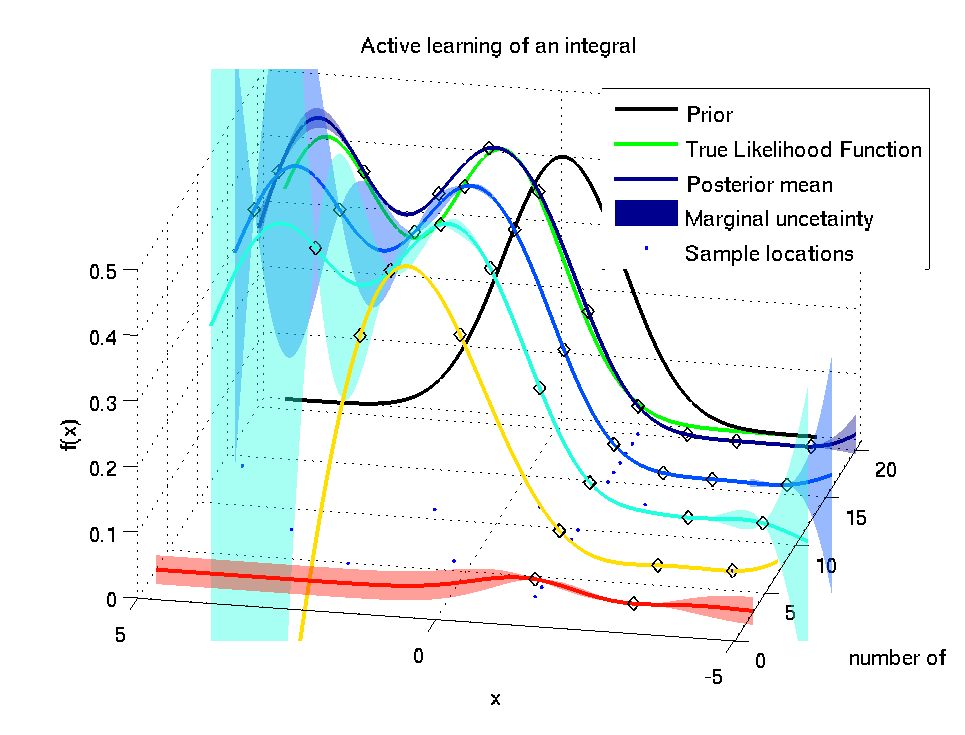
\includegraphics[width=0.48\textwidth]{figures/active_learning.eps}
%\caption{An example of the posterior over likelihood functions converging as new samples are selected.}
%\label{fig:active_learning}
%\end{figure}

\begin{figure}
\centering
\psfragfig{figures/plots/sampleplot_two_spikes_1d}
\caption{The location of samples chosen by different methods.}
\label{fig:sample_paths}
\end{figure}

Active sampling selects a new sample $\lfv_a$ so as to minimise the expected variance in the evidence after adding it to the model of $\ell$.  The objective is therefore to choose the $\lfv_a$ that minimizes the expected loss;
%
\begin{align}
\lfv_a = \argmin_{\lfv_a} \bigl\langle \cov{\If}{Z_0,\tvr_{s,a}}\mid Z_0,\tvr_{s}\bigr\rangle 
\end{align}
where the expected loss is
\begin{align}
&\bigl\langle \cov{\If}{Z_0,\tvr_{s,a}}\mid Z_0,\tvr_{s}\bigr\rangle 
\nonumber\\
% & = \secm{\inty{\lfn}}{Z_0,\tvr_s} 
% - \int\mean{\inty{\lfn}}{Z_0,\tvr_{a,s},\Delta_c}^2\nonumber\\
% & \hspace{3.8cm} \p{\tr_a}{\tvr_s}\ud\tr_a\,.\nonumber\\
 & = \secm{\If}{Z_0,\tvr_s} 
 - \int\mean{\If}{Z_0,\tvr_{a,s},\Delta_c}^2\nonumber\\
& \hspace{0.2cm}
\times\N{\tr_a}
{\hat{m}_a }
{\hat{C}_a +\pderiv{\hat{m}_a}{w}C_w\pderiv{\hat{m}\tra_a}{w}}
\ud\tr_a\,.\label{eq:exp_var}
\end{align}
and
\begin{align}
\hat{m}_a & \deq \mean{\tr_a}{\tvr_s,\hat{w}}\\ 
\hat{C}_a & \deq \cov{\tr_a}{\tvr_s,\hat{w}}\,.
\end{align}
The first term in \eqref{eq:exp_var}, the (expected) second moment, is independent of the selection of $\lfv_a$ and hence can be safely ignored for active sampling. This is true regardless of the probabilistic model chosen for the likelihood surface. 
Noting that $\int \exp(c\, y)\, \N{y}{m}{\sigma^2} \ud y = \exp(c\, m + \nicefrac{1}{2}\, c^2 \sigma^2)$, 
the second term, the negative expected squared mean, can be resolved analytically\footnote{We assume that $\Delta$ does not depend on $\tr_a$, only its location $x_a$: we know $\Delta(x_a) = 0$ and assume $\Delta$ elsewhere remains relatively unchanged.}
 for any trial $\lfv_a$ (we omit the laborious details of doing so). We do not have to make a linearisation approximation here, and the posterior over $\tr_a$ can be fully exploited for its most important purpose: selecting new samples. 

In order to minimize the expected variance, the objective in \eqref{eq:exp_var} encourages the maximization of the expected squared mean of $Z$. Due to our log-\gpb model, one means of doing so is to seek points where the log-likelihood is predicted to be large: exploitation.  The objective function in \eqref{eq:exp_var} also encourages the choice of points where our current variance in the log-likelihood is significant, leading to exploration. Note that our variance for $\tr_a$ has been inflated due to our consideration of the influence of hyperparameters (See Figure \ref{fig:integrate_hypers}), which we expect to promote additional exploration, as desired.



\section{Experiments}
\label{sec:experiments}

We now present empirical evaluation of the various components of our algorithm in a variety of different experiments.

\paragraph{Metrics:} We judged our methods according to three metrics, all averages over $N$ similar experiments indexed by $i$. Define $Z_i$ as the ground truth evidence for the $i$th experiment, $m(Z_i)$ as its estimated mean  and $V(Z_i)$  as its predicted variance. Firstly, we compute the normalised mean square error,
$
\acro{nmse} \deq 10 \log_{10} \nicefrac{1}{N} \sum_{i=1}^{N} \nicefrac{(m(Z_i) - Z_i)^2}{Z_i^2}\,,
$
providing some measure of the average percentage error, in decibels. Next we compute the log-density of the truth, assuming experiments are independent,
$
\log p(\vect{Z}) = \sum_i \log \N{Z_i}{m(Z_i)}{V(Z_i)}
$. This allows us to determine how accurate are our variance estimates. As a further metric, we supply the calibration $\mathcal{C}$, defined as the fraction of experiments in which the ground truth lay within our 50\% confidence interval $\bigl(m(Z_i) - 0.6745 \sqrt{V(Z_i)}, m(Z_i) + 0.6745 \sqrt{V(Z_i)}\bigr)$. Ideally, $\mathcal{C}$ would be exactly 50\%: any higher, and a method is under-confident, any lower and it is over-confident. 

\paragraph{Methods:} We firstly compared against simple Monte Carlo (\acro{smc}). \acro{smc} generates samples $x_1 \dots x_N$ from the prior distribution, and estimates $Z$ by $$\hat{Z} = \frac{1}{N} \sum_{n=1}^{N} \lfn(x_n).$$  An estimate of the variance of $\hat{Z}$ is given by the standard error of $\lfn({\bf x})$.

As an alternative Monte Carlo technique, we also implemented Annealed Importance Sampling (\acro{ais}) using a Metropolis-Hastings sampler.  The inverse temperature schedule was linear as in \citep{BZMonteCarlo}, and the proposal width was adjusted to attain approximately a 50\% acceptance rate.  In an attempt to be as generous to \acro{ais} as possible, the posterior variance of the \acro{ais} estimate of $Z$ was set to the empirical variance over 10 chains.  An alternative sampler which we did not use was Hamiltonian Monte Carlo, which uses information about the derivatives in order to speed mixing.  However, Bayesian Quadrature can also incorporate information about the derivatives of the likelihood function, and would presumably also perform better if given this information.  An exhaustive comparison of sampling methods is beyond the scope of this paper.

Our first model-based method was Bayesian Monte Carlo (\acro{bmc}) -- the algorithm used in \citep{BZMonteCarlo}, in which samples were drawn from the \acro{ais} chain just described, and a \gp was fit to the likelihood samples. For this \gp, and the others that follow, the hyperparameters were selected as those that maximised the likelihood. 

We then tested four novel methods. Firstly, Bayesian Quadrature (\acro{bq}), which employed the linearisation approach of Section \ref{sec:model_lik} to modeling the log-transformed likelihood values. The samples supplied to it were drawn from the same \acro{ais} chain as used above. \acro{bq}* is identical except that it additionally took the approach of Section \ref{sec:marginalizing} to approximately marginalising hyperparameters, where \acro{bq} did not. The performance of these methods allow us to quantify to what extent our innovations improve estimation given a fixed set of samples. 

Next, we tested a novel algorithm, Doubly Bayesian Quadrature (\acro{bbq}). The method is so named for the fact that we use not only Bayesian inference (with a \gpb over the log-transformed likelihood) to compute the posterior for the evidence, but also Bayesian decision theory to select our samples actively, as described in Section \ref{sec:BBQ}. Note that \eqref{eq:exp_var} was minimised using a multi-start local optimizer, where the starting points were chosen as $\lfv_c$. Finally, \acro{bbq}* was the same algorithm, but with hyperparameters  approximated marginalised. Both algorithms demonstrate the influence of active sampling on our performance. 

\paragraph{Problems:}
We chose a variety of problems which would demonstrate the strengths and weaknesses of the various methods we compared. Please refer to Table \ref{tbl:problem_descriptions} for brief descriptions of the likelihood functions chosen; for all problems, we assumed Gaussian priors. As in \citet{BZMonteCarlo} and \citet{BQR}, we focus on evaluating evidences given only low numbers of samples. We are motivated by real-world problems where evaluating likelihood samples is (computationally or otherwise) expensive, for which it is desirable to determine the techniques for evidence estimation that can operate best when permitted only a small number of samples. Ground truth $Z$ is available for only some integrals; for the non-analytic integrands, $Z$ was estimated by a run of \acro{smc} with $10^6$ samples.

% --- Automatically generated by print_problem_descriptions.m ---
% Exported at 21-Feb-2012 16:19:05
\begin{table}[h!]
\label{tbl:problem_descriptions}
\begin{center}
\begin{tabular}{ll}
 Problem name & Description \ 
 \\ \midrule 
easy 1d & A smooth 1D Gaussian. \\ 
bumpy 1d & a highly varying function \\ 
two spikes 1d & Two widely separated skinny humps \\ 
two hills 1d & Two smooth Gaussians \\ 
funnel 2d & Radford Neal's funnel plot \\ 
friedman 3d & isotropic BMC paper experiment. \\ 
easy 4d & A smooth 4D isotropic Gaussian. \\ 
two spikes 4d & Two widely separated skinny humps \\ 
two hills 4d & Two smooth Gaussian hills \\ 
friedman 7d & BMC paper experiment. \\ 
prawn 6d mean field & mean field model. \\ 
prawn 6d markov & best markovian model. \\ 
prawn 6d non-markov & best non-markovian model. \\ 
\end{tabular}
\end{center}
\end{table}
% End automatically generated LaTeX


Of particular note in Table \ref{tbl:problem_descriptions} is the funnel 2d example, drawn from \citet{NealMC}.This is known to be particularly challenging

We also reproduced an experiment from \citet{BZMonteCarlo}, in which we compute the evidence for a \gpb model for a synthetic function from \citet{friedman1991}. This required the marginalisation of seven inputs (friedman 7d); we also consider a restricted problem with only three inputs (friedman 3d). Note that $\gpb$ likelihoods are often expensive to compute, scaling as $N^3$ in the number of data $N$.

Finally, we compared approaches on a real scientific problem. Bayesian model comparison is emerging as an important method for comparing theories in the biological sciences 
\citep{penny2010comparing, mann2011bayesian, mann2011objectively, rosa2011bayesian}. \citet{mann2012multi} applied a model comparison methodology to discover the rules of interaction between simple individual animals (glass prawns, {\it Paratya australiensis}) which lead to coherent group motion. We aim to reproduce the experiments of \citep{mann2012multi} to calculate the evidence for each of three different models: a mean field model, a Markovian model and a non-Markovian model. Given the large corpus of data available, evaluating likelihood samples for these models is computationally demanding. For the purposes of our own experiments, we consider only a hundredth of the available data.


\paragraph{Evaluation}

%  \begin{figure}
%  \centering
%  \begin{tabular}{ccc}
%  	\psfragfig{figures/integrands/easy_1d} &
%  	\psfragfig{figures/integrands/bumpy_1d} 
%  	\psfragfig{figures/integrands/two_spikes_1d}
%  \end{tabular}
%  \caption{The one-dimensional integrands in our test suite.  Green dashed lines are priors, blue lines are likelihoods.
%  % \textcolor{red}{mike says: maybe we should make the lines variously dashed to help with B\&W printing. Also I'm not sure we need the posterior, which could be removed to de-clutter.}
%  }
%  \label{fig:1d_problems}
%  \end{figure}
% 
% %\begin{figure}
% %\centering
% %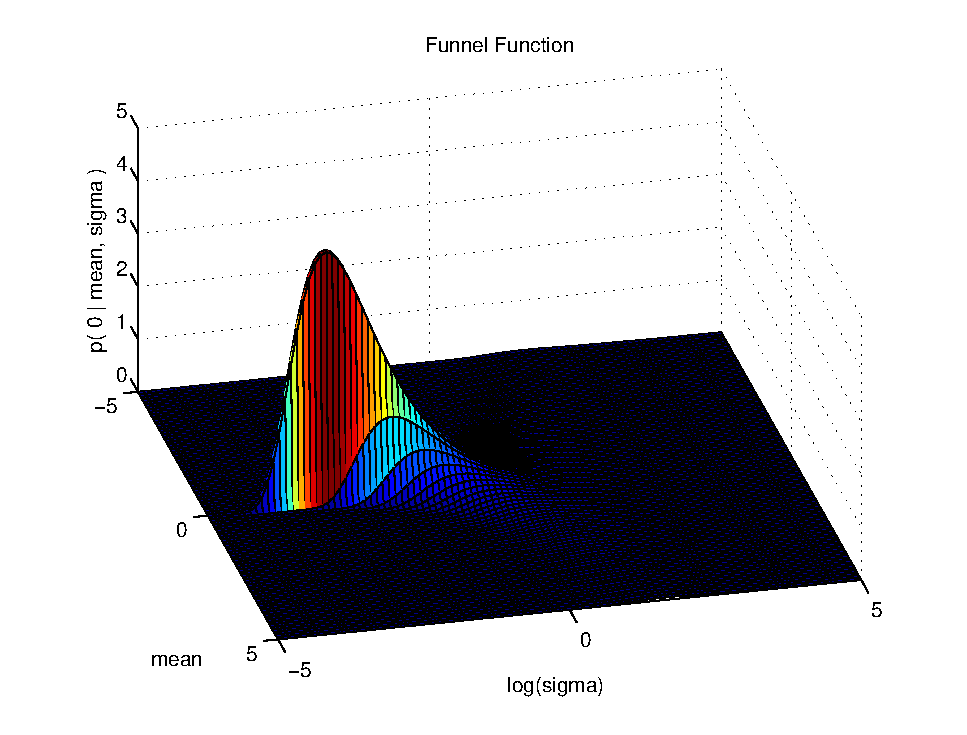
\includegraphics[width=0.45\textwidth]{figures/integrands/funnel.eps}
% %\caption{Radford Neal's funnel problem in 2 dimensions.}
% %\label{fig:funnel}
% %\end{figure}
% 
% %\begin{minipage}[t][0.45\paperheight][t]{0.45\paperwidth}
% %    % --- Automatically generated by latex_table.m ---
% Exported at 16-Feb-2012 13:24:18
\begin{table}[h!]
\caption{{\small
time taken (s)
}}
\label{tbl:time taken (s)}
\begin{center}
\begin{tabular}{l  r r r r r r r}
Integrand & \rotatebox{0}{ SMC }  & \rotatebox{0}{ AIS }  & \rotatebox{0}{ BMC AIS }  & \rotatebox{0}{ LBMC }  & \rotatebox{0}{ SBQ }  & \rotatebox{0}{ SBQ GPML }  & \rotatebox{0}{ BQ AIS }  \\ \midrule
simple & $\mathbf{0.023}$ & $1.306$ & $2.026$ & $1.251$ & $36.344$ & $12.158$ & $22.325$ \\
simple translated & $\mathbf{0.009}$ & $1.295$ & $1.948$ & $1.384$ & $ NaN$ & $ NaN$ & $23.192$ \\
simple scaled & $\mathbf{0.012}$ & $1.288$ & $1.897$ & $1.116$ & $37.762$ & $11.947$ & $21.611$ \\
easy 1d & $\mathbf{0.009}$ & $1.766$ & $2.064$ & $1.079$ & $45.821$ & $12.779$ & $ NaN$ \\
bumpy 1d & $\mathbf{0.007}$ & $1.126$ & $2.119$ & $1.144$ & $16.984$ & $26.335$ & $35.352$ \\
two spikes 1d & $\mathbf{0.016}$ & $2.781$ & $2.342$ & $1.888$ & $45.635$ & $ NaN$ & $45.693$ \\
two hills 1d & $\mathbf{0.020}$ & $2.781$ & $2.151$ & $1.091$ & $38.483$ & $11.402$ & $30.592$ \\
funnel 2d & $\mathbf{0.033}$ & $2.566$ & $2.241$ & $0.618$ & $67.442$ & $6.688$ & $9.770$ \\
friedman 3d & $\mathbf{0.371}$ & $12.441$ & $3.578$ & $0.447$ & $171.890$ & $7.807$ & $11.814$ \\
easy 4d & $\mathbf{0.010}$ & $1.924$ & $2.518$ & $0.666$ & $147.084$ & $10.071$ & $11.208$ \\
two spikes 4d & $\mathbf{0.012}$ & $2.997$ & $2.829$ & $ NaN$ & $ NaN$ & $ NaN$ & $ NaN$ \\
two hills 4d & $\mathbf{0.012}$ & $2.984$ & $2.321$ & $0.637$ & $219.580$ & $16.164$ & $11.057$ \\
friedman 7d & $\mathbf{0.356}$ & $11.618$ & $3.990$ & $4.756$ & $443.423$ & $57.409$ & $ NaN$ \\
\end{tabular}
\end{center}
\end{table}
% End automatically generated LaTeX

% %\end{minipage}
% 
% 
%\begin{figure}
%	\centering
%\end{figure}

\begin{figure}
	\centering
	\psfragfig[width=6cm,height=4cm]{figures/plots/log_of_truth_plot_simple} 	
	\psfragfig[width=3cm]{figures/plots/legend}
	\caption{The negative log density of the true normalization constant, versus different methods.}
\end{figure}

\begin{figure}
	\centering
	\psfragfig[width=8cm,height=6cm]{figures/plots/varplot_easy_4d}
	\caption{The posterior mean and variance over Z for different methods, compared to the true Z (in black)}
\end{figure}




\section{Discussion}

Adjusting the number of candidate points allows one to trade off between computational speed and number of samples required.

While we used an active learning scheme in this paper, Bayesian Quadrature can be used on samples generated by any method.

\paragraph{Future Work}There are many ways to improve the \gpb model used to model likelihood functions.  First and foremost, the Gaussian kernel used in this paper has very weak generalization abilities.  Allowing a richer class of kernels will allow the \gpb model to shrink its posterior much more quickly.  For example, log-likelihood functions typically take the form of a sum of many terms, each depending only on a small number of variables.  This prior information could easily be incorporated into the \gp, presumably allowing the \acro{bbq} algorithm to form concentrated posterior distributions over high-dimensional likelihoods.

The methods developed here can be applied without modification to discrete domains.

\section{Conclusions}

 In this paper, we have made several advances to the \acro{bmc} method.  We have also demonstrated the many advantages of model-based integration over standard \acro{mcmc}: a natural stopping criterion, an estimate of uncertainty in our integral, and the ability to use active learning to select our samples rather than Monte Carlo methods.

\acro{mcmc} is an extremely widely used method, and advances in \acro{mcmc} allow modelers [such as...] to use richer model classes and to be more confident in their model evaluations.  While we do not expect model-based integration approaches to be a better choice in every instance, we expect that this family of approaches will one day be seen as a standard alternative to \acro{mcmc}.

\section*{Acknowledgements}

\bibliography{bub}
\bibliographystyle{icml2012}
\pagebreak
% --- Automatically generated by latex_table.m ---
% Exported at 11-Feb-2012 20:59:11
\begin{table}[h!]
\caption{{\small
neg log density of truth at 100 samples
}}
\label{tbl:neg log density of truth at 100 samples}
\begin{center}
\begin{tabular}{l  r r r r r r}
Integrand & \rotatebox{0}{ SMC }  & \rotatebox{0}{ AIS }  & \rotatebox{0}{ BMC }  & \rotatebox{0}{ SBQ }  & \rotatebox{0}{ SBQ GPML }  & \rotatebox{0}{ BQ GPML AIS }  \\ \midrule
simple test & $-1.186$ & $233.335$ & $\mathbf{-2.942}$ & $-2.237$ & $-0.999$ & $-1.915$ \\
simple test transformed & $-1.186$ & $233.335$ & $\mathbf{-2.942}$ & $ NaN$ & $-1.104$ & $-1.915$ \\
easy 1d & $0.627$ & $\mathbf{-2.198}$ & $-1.189$ & $-0.453$ & $-1.145$ & $-1.353$ \\
bumpy 1d & $\mathbf{-3.050}$ & $>$ 1000 & $3.163$ & $-2.043$ & $ NaN$ & $0.867$ \\
bumpy 1d exp & $\mathbf{-3.518}$ & $>$ 1000 & $0.731$ & $-2.424$ & $ NaN$ & $0.015$ \\
two spikes 1d & $2.970$ & $24.156$ & $1.386$ & $ NaN$ & $\mathbf{0.120}$ & $1.220$ \\
two hills 1d & $2.970$ & $24.156$ & $1.386$ & $ NaN$ & $\mathbf{0.120}$ & $1.220$ \\
funnel 2d & $12.439$ & $52.654$ & $\mathbf{0.493}$ & $ NaN$ & $ NaN$ & $0.782$ \\
friedman 3d & $\mathbf{ NaN}$ & $ NaN$ & $ NaN$ & $ NaN$ & $ NaN$ & $ NaN$ \\
easy 4d & $0.601$ & $44.220$ & $0.410$ & $ NaN$ & $ NaN$ & $\mathbf{0.328}$ \\
two spikes 4d & $\mathbf{5.977}$ & $153.904$ & $23.489$ & $ NaN$ & $ NaN$ & $13.897$ \\
two hills 4d & $2.741$ & $687.308$ & $21.552$ & $ NaN$ & $ NaN$ & $\mathbf{0.356}$ \\
friedman 7d & $\mathbf{ NaN}$ & $ NaN$ & $ NaN$ & $ NaN$ & $ NaN$ & $ NaN$ \\
\end{tabular}
\end{center}
\end{table}
% End automatically generated LaTeX

% --- Automatically generated by latex_table.m ---
% Exported at 24-Feb-2012 15:01:01
\begin{table}[h!]
\caption{{\small
log squared error at 150 samples
}}
\label{tbl:log squared error at 150 samples}
\begin{center}
\begin{tabular}{l  r r r r r r r}
Integrand & \rotatebox{0}{ SMC }  & \rotatebox{0}{ AIS }  & \rotatebox{0}{ BMC }  & \rotatebox{0}{ BQ }  & \rotatebox{0}{ BQ* }  & \rotatebox{0}{ BBQ }  & \rotatebox{0}{ BBQ* }  \\ \midrule
simple & $-5.713$ & $-0.758$ & $-10.933$ & $-10.336$ & $-10.336$ & $-13.335$ & $\mathbf{-14.468}$ \\
bumpy 1d & $-4.859$ & $-6.866$ & $-3.286$ & $-3.466$ & $-3.466$ & $-2.594$ & $\mathbf{-10.106}$ \\
two spikes 1d & $-1.294$ & $\mathbf{-5.449}$ & $-0.821$ & $-0.574$ & $-0.574$ & $-1.724$ & $-3.628$ \\
two hills 1d & $-9.423$ & $-2.346$ & $-5.229$ & $-14.669$ & $-14.669$ & $\mathbf{-18.318}$ & $-18.317$ \\
funnel 2d & $-3.921$ & $-0.070$ & $-1.467$ & $-1.437$ & $-1.437$ & $-2.206$ & $\mathbf{-4.454}$ \\
easy 4d & $-6.665$ & $-4.655$ & $-4.073$ & $\mathbf{-6.785}$ & $-6.785$ & $-1.909$ & $-5.237$ \\
two spikes 4d & $-2.030$ & $3.664$ & $-3.540$ & $-2.275$ & $-2.275$ & $-2.322$ & $\mathbf{-4.772}$ \\
two hills 4d & $-0.707$ & $2.858$ & $-1.909$ & $-1.265$ & $-1.265$ & $-2.725$ & $\mathbf{-3.543}$ \\
real prawn 6d mean field & $\mathbf{-7.259}$ & $2.173$ & $-1.416$ & $-1.187$ & $-1.187$ & $2.084$ & $2.083$ \\
real prawn 6d markov & $\mathbf{-5.056}$ & $3.795$ & $3.000$ & $3.028$ & $3.028$ & $3.408$ & $3.412$ \\
real prawn 6d non-markov & $\mathbf{3.621}$ & $4.499$ & $3.710$ & $3.642$ & $3.642$ & $4.343$ & $4.346$ \\
\end{tabular}
\end{center}
\end{table}
% End automatically generated LaTeX


\end{document} 


